\documentclass[sigconf, nonacm]{acmart}

%%% do not modify the following VLDB block %%
%%% VLDB block start %%%
\usepackage{pvldb}
%%% VLDB block end %%%

\renewcommand\vldbdoi{XX.XX/XXX.XX}
\renewcommand\vldbpages{XXX-XXX}
\renewcommand\vldbavailabilityurl{https://github.com/angelkurten/keel}

\usepackage{array}
\usepackage{makecell}
\usepackage{tabularx}
\usepackage{enumitem}
\usepackage{listings}
\usepackage[font=small,labelfont=bf]{caption}
\graphicspath{{./}}

\newcolumntype{L}{>{\raggedright\arraybackslash}X}
\newcolumntype{R}{>{\raggedleft\arraybackslash}X}
\newcolumntype{P}[1]{>{\raggedright\arraybackslash}p{#1}}
\newcolumntype{Q}[1]{>{\raggedleft\arraybackslash}p{#1}}
\lstset{basicstyle=\footnotesize\ttfamily,breaklines=true,breakatwhitespace=true,breakindent=1.5em,
  columns=fullflexible,keepspaces=true,upquote=true,xleftmargin=0pt,aboveskip=4pt,belowskip=6pt}
\newcommand{\code}[1]{\texttt{#1}}
\setlength{\emergencystretch}{2em}
\newcommand{\keelfig}[2]{\includegraphics[width=\linewidth]{#1}}

\usepackage{xr}
\externaldocument{supplement}
\begin{document}
\title{Keel: Compiling a Product's Events into Bitemporal Context for Agents}

\author{Angel K\"urten}
\affiliation{%
  \institution{Independent researcher}
  \city{Valledupar}
  \country{Colombia}
}
\email{angel@angelkurten.com}

\begin{abstract}
Agents inside a product ask what holds now, what held at an instant, and what the product had recorded by then. Keel answers from the product's own events. A cartridge declares a domain's event types, entity kinds, facts, relations and rules once; a deterministic ingest with no LLM builds a bitemporal graph per tenant whose transaction time comes from the events, so replaying the log in any order rebuilds it identically. The same cartridge compiles to two interfaces: five tools an agent calls, and bitemporal SQL views and rule macros that an optional read-only \code{query} tool serves, bound to the tenant by the store. We evaluate on temporal questions over eight real Jira projects of seven instances, in three sets: a development set, a pre-registered held-out set and a pre-registered confirmation set (1,032 questions, gold computed by an independent oracle from the log). Hand-written bitemporal SQL over the log is the strongest baseline. On the held-out set, as registered, Keel's core read tools trail it by 2.8 points (95\% CI $[-4.7, -1.4]$) while leading the product's API by 9.1. Two conditions built after that result, the SQL compiled from the cartridge and the core tools plus \code{query}, tied it there and on the development set. Registered in advance on a third set (two projects of one Jira instance), both are not worse than hand-written SQL ($+0.3$ points, $[-0.3, +0.7]$, margin $-2$), and \code{query} adds 1.2 points to the core tools ($[+0.2, +2.5]$); the tools with \code{query} also cost the least per correct answer. That benchmark sits near its ceiling: every SQL-backed condition answers 96 to 99\%. On a harder slice of 320 questions registered afterwards, which combine two steps each, neither tie is confirmed (compiled SQL $-1.1$ points, $[-3.1, +0.8]$; tools with \code{query} $-1.6$, $[-3.8, +0.5]$), while \code{query} still adds 3.2 points to the core tools. With one agent, a domain declared once matched SQL written by hand on near-ceiling questions, and came within 2 points of it, not provably, on harder ones.
\end{abstract}

\maketitle

%%% do not modify the following VLDB block %%
%%% VLDB block start %%%
\vldbtopmatter
%%% VLDB block end %%%

\section{Introduction}
\label{sec:intro}

An agent shipped inside a product, a support copilot or a planning assistant, needs the product's state: what a customer has, what changed, what was true when something happened, what the product had recorded at that moment, and which business rule applies. Each team that ships such an agent rebuilds the same pipeline from the product's database to the agent's prompt. Memory systems for agents answer part of this, but they build memory from conversation: an LLM reads text and writes facts \cite{mem0,zep}. A product already holds its facts as events with time. Event sourcing and change data capture derive application state from those events \cite{fowler-es,debezium}, and temporal databases have long answered as-of and as-known-at queries \cite{jensen-glossary,snodgrass-book}.

Keel puts the two together for agents. A \emph{cartridge} declares a domain once: its event types, entity kinds and their facts, relations, rules and memory policy, plus handlers of about ten lines that map each event to five store primitives. A deterministic ingest, with no LLM and no network call, builds a bitemporal graph per tenant whose transaction time is the one the event's source declares, so a replay of the log in any order rebuilds the same graph, transaction time included. From the same cartridge Keel compiles two interfaces. One is five tools (\code{context}, \code{history}, \code{search}, \code{related}, \code{annotate}) whose results carry rule verdicts, counts and changes. The other is bitemporal SQL: point-in-time views per entity kind, a change view and one macro per rule, in three dialects, which an optional sixth tool, \code{query}, serves read-only and bound to one tenant by the store, never by the agent's SQL.

Whether that is worth doing is an empirical question with an obvious baseline: a database engineer who models the same log in bitemporal tables and writes the point-in-time views and rule macros by hand. We built that baseline ourselves, to the textbook construction; on the development set it scored above Keel's tools (99.3\% against 97.1\%). This paper reports how Keel fares against it on data development never saw, in three stages: a development set; a held-out set whose tenants, conditions, budget and analysis were registered before any run; and, because the two conditions that tied hand-written SQL on the held-out set were built after reading its results, a third, confirmation set registered in advance with three hypotheses and their decision rules. Because those sets sit near their ceiling, a fourth stage registered a harder slice over the same tenants with the same hypotheses. The registered held-out result was negative for Keel's core tools, the hard slice's for the two ties, and we report both as such.

Contributions:

\begin{enumerate}[leftmargin=*]
\item \textbf{One declaration, two compiled interfaces (C1).} A cartridge compiles to agent tools and to bitemporal SQL (Section~\ref{sec:compile}); the SQL comes with the paragraph that documents it for an agent, generated from the same declaration. The core names no domain: five example cartridges, a Jira cartridge and a cartridge over a third-party benchmark's tables (TDBench \cite{tdbench}) run with no domain-specific code under \code{keel/}.
\item \textbf{Source-declared transaction time, order-independent (C2).} A formal model (Section~\ref{sec:formal}) in which every fact's position in its history is a function of fields it carries, so any permutation of the log yields the same graph and the same answer to ``what held at $a$, as known at $k$''; checked on real and synthetic logs.
\item \textbf{A benchmark and a staged protocol (C3).} Temporal questions over real Jira projects with injected late arrivals and corrections, gold from an oracle that imports nothing from Keel, and three sets: development, pre-registered held-out, pre-registered confirmation, plus a pre-registered harder slice (Section~\ref{sec:benchmark}).
\item \textbf{What the compiled interfaces buy (C4).} The SQL compiled from the cartridge is not worse than hand-written SQL, and Keel's tools with \code{query} are not worse either, both confirmed on the third set but not on the harder slice, where hand-written SQL leads by 1 to 2 points; the core tools alone trail hand-written SQL, lead the product's API, and gain from \code{query} on every set (Section~\ref{sec:results}).
\end{enumerate}

The first version of this work compared Keel's five tools with the product's API, retrieval and memory systems built by LLM extraction on the development set, and measured governed write-back by agents. Those results stand as development-set results; Section~\ref{sec:firstrun} summarizes them and Appendix~\ref{app:dev} gives them in full.

% ===========================================================================
\section{Model}
\label{sec:model}

Keel turns a product's events into a bitemporal graph per tenant, with no LLM, and serves it through tools and SQL compiled from the same cartridge (Figure~\ref{fig:1}).

\begin{figure*}[t]
\centering
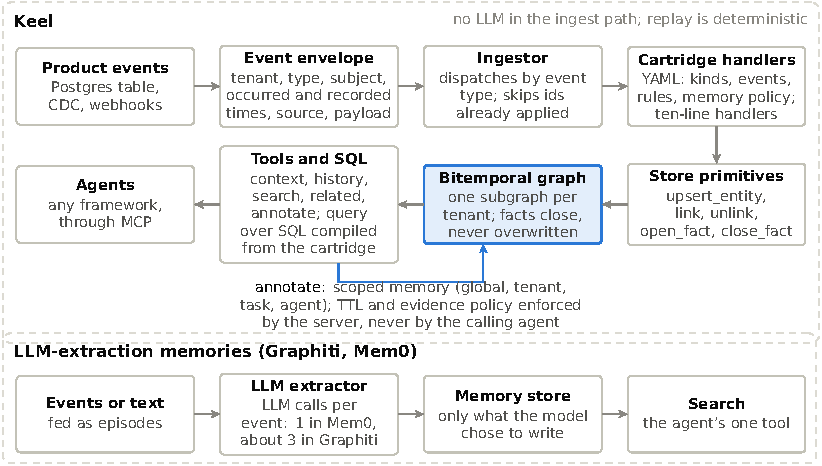
\includegraphics[width=5.5in]{figures/fig1-architecture.pdf}
\caption{Keel (top): product events through cartridge handlers into a bitemporal graph per tenant, read through tools and SQL compiled from the cartridge and written back only through annotate; memories built by LLM extraction (bottom) put a model between the event and what is stored.}
\label{fig:1}
\end{figure*}

\textbf{Events and cartridges.} An event carries a tenant, a type, a subject (\code{<kind>:<id>}), when it happened (\code{occurred\_at}), when its source recorded it (\code{recorded\_at}), a source and a payload. A cartridge declares the domain: entity kinds and, per kind, its facts and the few attributes a tool needs to label an entity; relations, with \code{one: true} for a relation an entity has at most one of; the event catalog with payload types; rules; and memory policy. Handlers map a payload to five primitives (\code{upsert\_entity}, \code{link}, \code{unlink}, \code{open\_fact}, \code{close\_fact}). The Jira cartridge of Section~\ref{sec:benchmark} is 104 lines of YAML and 58 of Python. The core, under \code{keel/}, names no kind, relation, predicate, rule or event type; an entity carries a pointer to its row in the system of record, not a copy of it.

\textbf{Rules.} A rule applies to one kind and is a tree of conditions on facts (comparisons and membership, a null value included), composed with \code{all}, \code{any} and \code{not}, following a relation in either direction (\code{via}) to a condition on the neighbour, and measuring how long a value has held, in days or business days (\code{open\_for\_days} and its kin). Rules are evaluated when a tool or a query reads, at the instant and knowledge time it reads at, and never materialized at ingest. What they cannot express, counts over time or aggregates, stays a definition the agent applies.

\textbf{Bitemporal facts, transaction time from the event.} A fact carries valid time (when it held in the world) and transaction time (when the product recorded it). An event that declares \code{recorded\_at} writes with it, so replay rebuilds when each fact was learned and a late event keeps its own time; a separate ingest-clock stamp (\code{changed\_at}) drives the change feed and is never a query time. Facts close; a handler never overwrites or deletes one.

\subsection{Formal model}
\label{sec:formal}

A fact is a tuple with its subject, predicate, value, valid start, recording time and the event that set it; its valid end and the time that end was learned are derived, never written by a handler:
\begin{equation*}
f = \langle s,\ p,\ v,\ t^{v}_f,\ t^{r}_f,\ e_f \rangle
\end{equation*}
Here $t^{r}_f$ is the recording time the source declares on the event, not the store's clock, so a replay reproduces it; Keel takes the source's word for it, and a source that lies about it misleads every reader alike. Facts of one subject and predicate form a \emph{slot} (a predicate the cartridge declares multi-valued has one slot per author, so authors never close each other's facts); they are ordered by a total order on what they carry, never on arrival:
\begin{equation*}
f \prec g \iff \big(t^{v}_f,\ t^{r}_f,\ e_f,\ v_f\big) <_{\mathrm{lex}} \big(t^{v}_g,\ t^{r}_g,\ e_g,\ v_g\big)
\end{equation*}
Knowledge at transaction time $k$ is the set of facts recorded by then, $K_k = \{\, f \mid t^{r}_f \le k \,\}$. Within a slot, a fact holds until the next fact of $K_k$ starts, or until an explicit close mark $c \in K_k$ that covers it (a close mark is a fact of the slot written by \code{close\_fact}, with its own valid and recording time, that ends the fact current at its valid time instead of starting a value):
\begin{equation*}
\mathit{end}_k(f) = \min\big(\{\, t^{v}_g \mid g \in K_k,\ f \prec g \,\} \cup \{\, t^{v}_c \mid c \in K_k \text{ closes } f \,\}\big)
\end{equation*}
with $\min \emptyset = \infty$. The answer to ``what held at world time $a$, as known at $k$'' (Figure~\ref{fig:2}) is
\begin{equation*}
F(a, k) = \{\, f \in K_k \mid t^{v}_f \le a < \mathit{end}_k(f) \,\},
\end{equation*}
and with $k$ omitted, $k = \infty$: every fact is known. The stored row caches $\mathit{end}_\infty(f)$ as \code{valid\_to}, and when that end was learned, $\max(t^{r}_f, t^{r}_g)$ for the fact $g$ that ends it, as \code{closed\_at}. A known-at read recomputes $\mathit{end}_k$ rather than read the cached end, since a fact recorded after $k$ may have moved it (a late fact landing between two known ones). A value recorded wrong and corrected later shares its valid start with the correction and precedes it in $\prec$, so its valid interval is empty under full knowledge and it answers only known-at reads before the correction, which corresponds to a logically deleted row in a bitemporal table \cite{snodgrass-book}.

\textbf{Order independence.} \emph{For any permutation of a log, ingest builds the same facts and relations, and $F(a,k)$ is the same for every $a$ and $k$.} Entity attributes are outside it: \code{upsert\_entity} merges them last-arrival-wins, so a cartridge whose handlers write an attribute more than once must not depend on its order (the Jira cartridge writes them only at creation). $K_k$ is a set defined by the facts' own recording times; $\prec$ is a total order on fields every fact carries; so $\mathit{end}_k$ and $F$ are functions of the set of facts, and the cached ends are $\mathit{end}_\infty$ and the recording times of two facts of that set. Ingest skips event ids it has applied, so duplicates do not change the set. Relations follow the same rule: a link's interval is a function of its link and unlink events, whatever order they arrive in. This is the usual requirement of a deterministic projection \cite{cedr,mcsherry-dd}; what Keel adds is that transaction time is included, because the source declares it. The argument covers the definition; that each store's incremental maintenance of the cache matches it is checked empirically, not proved: a conformance suite every store runs checks that every arrival order of a late fact landing between two known ones gives the same known-at answers, and Section~\ref{sec:determinism} compares whole graphs.

\begin{figure}[t]
\centering
\keelfig{figures/fig2-bitemporal.pdf}{2}
\caption{One field's versions in valid time (across) and recorded time (up). B arrives late: it holds from its world time but is known only from when it was recorded. C is recorded with a wrong value and later corrected to D; nothing is overwritten. A vertical line is an as-of read at $a'$ with all knowledge (D); the point at $k$ is a known-at read, what was believed then (C).}
\label{fig:2}
\end{figure}

% ===========================================================================
\section{Compiling a cartridge}
\label{sec:compile}

\subsection{To tools}
\label{sec:tools}

\code{context} reads a subject now, at \code{as\_of}, or as known at \code{as\_known\_at}, with its facts, relations and rule verdicts. \code{history} returns a subject's facts over time, or the tenant's changes in a world-time window. \code{search} lists a kind by text, by fact values (\code{where}) or by rule at an instant, as known at an instant, with counts. \code{related} returns neighbours by relation at an instant, and \code{annotate} writes governed memory (Section~\ref{sec:memory-gov}). The tools are typed by the cartridge: a predicate, relation or rule the cartridge does not declare is refused with the names it does. Their replies are shaped for an agent's context: a brief form by default (a fuller one on request), a compact text rendering over MCP whose structured content stays the contract, counts before listings, and a listing ceiling that says what it cut. In the development set's ablations (Appendix~\ref{sec:ablations}) the brief form cut the cost per correct answer on tenant-wide questions 7 to 21 times and the ceiling about 4 times, with accuracy within noise.

\subsection{To SQL}
\label{sec:sql}

\code{keel.sqlgen.generate} compiles a cartridge to SQL text, deterministically and with no model: the same cartridge always yields the same text. The tables are the SQL stores' own (\code{entities}, \code{facts}, \code{relations}); over them it emits, as table macros (DuckDB), set-returning functions (Postgres) or queries inlined at call time (SQLite, which has no table macros):

\begin{itemize}[leftmargin=*]
\item \code{facts\_known\_at(tenant, t, k)} and \code{state\_known\_at}, $F(t, k)$ of Section~\ref{sec:formal} with $\mathit{end}_k$ recomputed in SQL from the facts recorded by $k$, and the visibility rules for memory scopes; \code{state\_at} is the same with $k = \infty$.
\item Per entity kind that declares its facts, \code{<kind>\_state\_at(tenant, t)} and \code{<kind>\_state\_known\_at(tenant, t, k)}: one row per entity, one decoded column per declared fact, \code{<fact>\_since} for each (when the value began), its attributes, and the target's id for each \code{one} relation.
\item \code{<kind>\_changes(tenant, since, until, k)}: one row per change of a declared fact in a world-time window, with old and new value, as \code{history} reports a change (a first value is not a change, nor a value recorded wrong and corrected later).
\item \code{relations\_at} and \code{relations\_known\_at}.
\item Per rule, \code{<rule>\_verdicts(tenant, t, k)} (true, false or null for every entity of its kind) and \code{<rule>\_at(tenant, t, k)} (the entities it holds for), compiled from the rule tree: \code{all}/\code{any}/\code{not} to three-valued boolean expressions, \code{via} to a join over \code{relations\_known\_at}, durations to differences of \code{<fact>\_since}.
\end{itemize}

\code{keel.sqlgen.describe} writes, from the same cartridge, the paragraph that tells an agent what all of this is: the views and their columns with each fact's description, which arguments are valid and which transaction time, the relations with their direction, each rule with its definition, and that macros take the tenant first and no schema prefix. For Jira the generator emits 118 lines of DuckDB (17 kB) and a paragraph of 802 tokens at release 0.36.0 (712 in the held-out run, before two fixes lengthened it); the hand-written baseline of Section~\ref{sec:conditions} is 361 lines of Python and SQL written for Jira (307 without blanks and comments), with a 695-token paragraph. The compiled SQL reaches every gold answer of the development and held-out sets with one query per question, and the stores answer tenant-wide tool calls through the same compiled rules (push-down): on all the tool calls behind the development set's 387 questions, the outputs are the same bytes on SQLite, DuckDB and Postgres as Keel's Python evaluation.

\subsection{The query tool}
\label{sec:query}

\code{query} takes one read-only statement (\code{SELECT} or \code{WITH}) over the compiled views and returns at most 200 rows by default, saying when it cut, within a timeout (5 s by default). It is off unless the host enables it, and complements the five tools rather than replacing them. The agent's SQL never binds the tenant; the store does:

\begin{itemize}[leftmargin=*]
\item \textbf{SQLite and DuckDB} answer from a per-tenant sandbox: a separate in-memory database holding a copy of only what the tenant may read (its accepted tenant-scope facts, its partition's share of global facts, its entities and relations), with the compiled views over it, rebuilt when the tenant's rows change. The copy is refused above 100,000 rows; such tenants are served from Postgres.
\item \textbf{Postgres} gives each tenant a login role of its own that reads only security-barrier views filtered by \code{current\_user}, which a session logged in as that role cannot change; each query runs in a transaction rolled back after it, under a statement timeout.
\end{itemize}

Agent and task memory and proposals are never in what \code{query} reads: the store cannot apply \code{Tools}' per-caller visibility to arbitrary SQL, so it leaves them out. Sixty tests cover the tool, its sandboxes, its security and its transports, among them attempts to read another tenant through every generated view and macro and the base tables, and to reach the catalogs, file and network functions, extension loading and \code{ATTACH}.

\subsection{Governed memory}
\label{sec:memory-gov}

Agents write back only through \code{annotate}, into scopes (global, tenant, task, agent) whose TTL and evidence policy the server enforces; a per-agent registry declared in the cartridge limits which scopes each agent writes and which kinds and relations it reads; a write to a wider scope can be filed as a proposal that changes no fact. Annotations are not events, so replay keeps them and rebuilds around them. Section~\ref{sec:firstrun} summarizes what this holds against; this paper's question sets do not exercise it (Section~\ref{sec:conditions}).

% ===========================================================================
\section{Benchmark}
\label{sec:benchmark}

\textbf{Data.} The Public Jira Dataset of Montgomery, Lüders and Maalej \cite{jira} (MSR 2022, CC BY 4.0) holds 16 public Jira instances. A tenant is one whole project. An adapter turns each issue's changelog into events: it names field values by their id as it stands today, keeps a link only while its adds outnumber its removes, files moved issues under their final key and anonymizes people as \code{user-<8 hex>}. A check replays the events and compares every issue's status, assignee, priority, resolution, type and links with Jira's current fields.

\textbf{Transaction time, injected.} Jira records when a change happened, not when anyone learned it. With a fixed seed, 5\% of eligible changes reach the log 1 hour to 30 days late, and 2\% are first recorded with a wrong value and corrected later; each injection leaves a window in which the value as recorded differs from the value as it happened.

\textbf{Questions.} Templates in seven types, filled with a fixed seed, with instants at least an hour from any change the question reads (Table~\ref{tab:questions}; templates in Appendix~\ref{app:templates}). Each tenant gets 129 questions: 105 about one issue and 24 tenant-wide. Gold comes from an oracle that rebuilds each tenant's history from the log alone and imports nothing from Keel. On the development set, a sample of gold answers was also rebuilt from the raw Jira export rather than the event log, by independent agents and by a person; it exposed one adapter bug (duplicate link adds), since fixed, and the records of that review are not part of the released artifacts.With no agent, Keel's primitives reach every set's gold; on the development and held-out sets so do one hand-written SQL query per question over the baseline's tables and one per question over the compiled SQL.

\begin{table*}[t]
\caption{Question types, with the number per tenant, what each asks and the form of its gold.}
\label{tab:questions}
\centering
\small
\begin{tabularx}{\textwidth}{l r L P{0.85in}}
\toprule
Type & Per tenant & Asks & Gold \\
\midrule
Current & 20 & A field's value now & Value \\
As-of & 25 & A field's value at an instant inside its history (80\% differ from today's) & Value \\
Known-at & 25 & A field's value at an instant, as recorded by a later instant & Value \\
Links & 15 & Of the issues linked to one by a relation at an instant, which were done & Set of keys \\
Rule & 15 & blocked, stalled or urgent\_unassigned at an instant, the definition given & Yes/no \\
Abstain & 5 & An issue that never existed, or one before it was created & Unknown \\
Tenant & 24 & Tenant-wide: issues with a status at an instant, counts, rule listings, changes in a window, sets as recorded by a later instant & Set or count \\
\bottomrule
\end{tabularx}
\end{table*}

\subsection{Three sets}
\label{sec:sets}

The sets share the pipeline, the templates and the per-type counts, and differ in instances, projects and seed (Table~\ref{tab:sets}).

\begin{table*}[t]
\caption{The three question sets. Tenants are whole projects; no instance is shared between sets.}
\label{tab:sets}
\centering
\footnotesize
\begin{tabularx}{\textwidth}{l L r r L}
\toprule
Set & Tenants (instance project, issues) & Questions & Seed & Status \\
\midrule
Development & Hyperledger INDY 2,323; MariaDB MXS 3,333; Spring SEC 3,150 & 387 & 7 & Read while Keel was tuned: tool descriptions, compact text, the generated views \\
\addlinespace
Held-out & JiraEcosystem AC 1,544; Sakai GRBK 1,433; RedHat PROJQUAY 2,455 & 387 & 31 & Tenants, conditions, commands, budget and analysis registered on 2026-10-26, before any run \\
\addlinespace
Confirmation & Apache TAJO 2,183; Apache RAVE 1,286 & 258 & 47 & Tenant rule, conditions, three hypotheses with margins, commands and analysis registered on 2026-11-01, before any question existed; two amendments before any of its questions existed, a third during the run (Section~\ref{sec:conditions}) \\
\bottomrule
\end{tabularx}
\end{table*}

\textbf{Selection.} Held-out tenants were chosen by a rule fixed before screening: 900 to 4,000 issues; the replay check mismatching on at most 1\% of issues; a priority scheme with Blocker, Critical or Highest, so the urgent rule can hold; at most 1\% of status values without a category; and the unmodified pipeline filling every per-type count. Of 97 projects in 11 instances, three passed, one per instance, and those are the set. The confirmation set's rule relaxed only the last condition (at least 100 questions and half of each type's count) and took the three passing projects with the most questions, at most one per instance. No project of the eight instances first named passed; an amendment, written before any question was generated, admitted every unused project, and none passed either. After the first amendment's question counts had been seen, and after the registration had said no further amendment would be made, a second amendment, written before Apache or Mojang (the two largest instances, left out of the earlier screenings for size) were restored, admitted their projects and added one rule: with fewer than three instances passing, fill to three by the same ranking, at most two per instance. Sixty Apache projects passed; Mojang's one candidate did not; the ranking gave TAJO and RAVE, the two Apache projects with all 129 questions, no replay mismatch and the most issues. The set is therefore disjoint from the other two in instances, projects and questions, but its two tenants share an instance; \code{evals/jira/confirm/README.md} records every step.

% ===========================================================================
\section{Conditions and protocol}
\label{sec:conditions}
\label{sec:systems}

Every condition reads the same log, late arrivals and corrections included; agents differ only in their tools and one paragraph of the system prompt that describes them (Table~\ref{tab:conditions}).

\begin{table*}[t]
\caption{Conditions. The \code{sql*} conditions run DuckDB 2.0.0 and \code{keel+query}'s \code{query} runs SQLite; all read-only, rows capped at 200 with the cut said, like Keel's listing ceiling.}
\label{tab:conditions}
\centering
\footnotesize
\begin{tabularx}{\textwidth}{P{0.75in} L P{1.5in}}
\toprule
Condition & What the agent gets & Sets \\
\midrule
\code{keel} & Keel's core tools over MCP, the four that read (\code{annotate} off), compact text, listing ceiling 200 & All three \\
\code{keel+query} & The same plus \code{query} over the SQL compiled from the cartridge, served by Keel's MCP server over an in-memory SQLite store; the compiled paragraph in the server's instructions & All three (post hoc on the first two) \\
\code{sql} & \code{sql\_query} over the log modelled by hand: one row per issue, each field's history as an SQL:2011-style bitemporal table, links bitemporal the same way, statuses and their categories, the raw events; and hand-written macros \code{issue\_state\_at(t)}, \code{issue\_state\_known\_at(t, k)}, \code{links\_at(t)} and one per rule & All three \\
\code{sql-tables} & The same tables without the macros; the rules as definitions in words & Held-out \\
\code{sqlgen} & \code{sql\_query} over Keel's own tables with the first generator's output: \code{state\_at}, \code{state\_known\_at}, \code{relations\_at} and the rule macros; a hand-written paragraph & Held-out \\
\code{sqlgen2} & The same with the per-kind and change views of Section~\ref{sec:sql}, and the paragraph generated by \code{describe} & All three (post hoc on the first two) \\
\code{api} & A Jira-like API: \code{get\_issue}, \code{get\_changelog} (both times, initial values) and \code{search\_issues} with JQL's \code{WAS\,\ldots\,ON} and \code{CHANGED DURING} (Appendix~\ref{app:apitools}) & Held-out (and the first run) \\
\bottomrule
\end{tabularx}
\end{table*}

\textbf{Agent.} Claude Haiku 5.5, three repetitions per condition, at its default temperature (callers cannot change it), thinking off, prompt caching on. The held-out registration named GPT-6 Luna too; an amendment before any run dropped it. Held-out and confirmation runs go straight to Anthropic's API; the development-set runs of \code{keel+query} and \code{sqlgen2} went through a gateway (OfoxAI) at a time the direct account had no credit, so their costs are not comparable with the other sets'. The confirmation run started through the gateway and, after 82 runs, was restarted from nothing straight to Anthropic, its route on the held-out set; the 82 rows are kept aside, unanalysed (the third amendment).

\textbf{Grading.} Every answer is structured: the agent ends with \code{ANSWER: <json>}, graded by exact match after normalizing case, empty values, issue-key prefixes and yes/no. No judge model is used; a set must match exactly. A run that ends in an error counts as wrong; a run lost to a gateway or network fault is set aside and asked again.

\textbf{Statistics.} Accuracy is the share of runs graded correct, a question's repetitions averaged first:
\begin{equation*}
\mathrm{Acc}(S) = \frac{1}{|Q|\,R} \sum_{q \in Q} \sum_{r=1}^{R} g\big(a_{q,r},\ \mathrm{gold}_q\big).
\end{equation*}
Questions of one tenant and type share a template and an issue population, so they are not independent draws. Intervals and differences use a cluster bootstrap that resamples tenant $\times$ type cells whole (tenant-wide questions by sub-type), $B = 10{,}000$, seed 0; a difference between two conditions is paired over the questions both answered. On the held-out set the five registered comparisons are tested two-sided with Holm's adjustment (the result files also give the bootstrap over questions as independent draws). On the confirmation set each hypothesis is a decision on the 95\% interval fixed in advance: \emph{H1}, \code{sqlgen2} $-$ \code{sql}, and \emph{H2}, \code{keel+query} $-$ \code{sql}, are confirmed if the interval's lower bound is above $-2$ points (non-inferiority); \emph{H3}, \code{keel+query} $-$ \code{keel}, if it is above 0. The 2-point margin was a practical tolerance fixed before the run, about 5 of the set's 258 questions; it is smaller than every significant gap the registered held-out comparisons found (2.8 to 9.1 points), but it was not derived from a cost model. No multiplicity adjustment: three claims, each stated in advance. Cost is the dollars spent over the correct runs, at the provider's prices.

\textbf{Code.} Held-out rows ran on four commits of \code{keel/}: d7b3576 for the registered conditions, 89e8510 for the zone-fixed \code{sqlgen}, 1cca5aa for \code{sqlgen2} and 25979b2 for \code{keel+query}; the confirmation set's on \code{keel/} as of d620fcb (release 0.36.0). Every result row records the repository commit, package versions and one flag for uncommitted changes under \code{keel/} or the harness; the flag is set on most held-out and confirmation rows, so the commit alone does not prove what ran.

% ===========================================================================
\section{Results}
\label{sec:results}

\subsection{Held-out set, as registered}
\label{sec:heldout}

As registered, Keel's core tools trail hand-written SQL by 2.8 points, tie hand-written SQL without its macros, and lead the product's API by 9.1 (Tables~\ref{tab:heldout} and~\ref{tab:planned}).

\begin{table}[t]
\caption{Held-out set, Haiku, 387 questions, three repetitions: accuracy (\%) with 95\% cluster CI, by scope, USD per correct answer and input tokens per run. Rows below the rule were built after the registered results were read.}
\label{tab:heldout}
\centering
\footnotesize
\setlength{\tabcolsep}{2.6pt}
\begin{tabular}{l r c r r r r}
\toprule
Condition & Acc. & 95\% CI & One & Tenant & USD/corr. & Tokens \\
\midrule
\code{api} & 86.7 & [79.3, 92.7] & 92.5 & 61.6 & 0.00087 & 9.9k \\
\code{keel} & 95.9 & [93.8, 97.6] & 96.9 & 91.2 & 0.00057 & 8.4k \\
\code{sql-tables} & 96.2 & [93.6, 98.3] & 97.6 & 90.3 & 0.00073 & 8.2k \\
\code{sqlgen}, registered & 89.6 & [81.4, 96.1] & 91.4 & 81.5 & 0.00085 & 9.9k \\
\code{sqlgen}, zone fixed & 98.2 & [96.6, 99.5] & 98.7 & 95.8 & 0.00075 & 10.1k \\
\code{sql} & 98.7 & [97.5, 99.6] & 98.4 & 100.0 & 0.00047 & 5.3k \\
\midrule
\code{sqlgen2} & 99.1 & [97.8, 100.0] & 98.8 & 100.0 & 0.00047 & 6.3k \\
\code{keel+query} & 99.1 & [97.9, 100.0] & 99.0 & 99.5 & 0.00043 & 9.7k \\
\bottomrule
\end{tabular}
\end{table}

\begin{table}[t]
\caption{Held-out set, the five registered comparisons: paired difference in points, 95\% cluster CI, Holm-adjusted $p$, and questions where A / B is better.}
\label{tab:planned}
\centering
\footnotesize
\setlength{\tabcolsep}{3pt}
\begin{tabular}{l r c r r}
\toprule
A $-$ B & Diff. & 95\% CI & $p_{\mathrm{Holm}}$ & A / B \\
\midrule
\code{keel} $-$ \code{sql} & $-2.8$ & [$-4.7$, $-1.4$] & $<0.001$ & 5 / 29 \\
\code{keel} $-$ \code{sqlgen} & $+6.3$ & [$+0.4$, $+13.9$] & 0.066 & 46 / 14 \\
\code{keel} $-$ \code{sql-tables} & $-0.3$ & [$-2.9$, $+2.2$] & 0.74 & 18 / 25 \\
\code{keel} $-$ \code{api} & $+9.1$ & [$+3.3$, $+16.4$] & $<0.001$ & 70 / 22 \\
\code{sql} $-$ \code{sqlgen} & $+9.1$ & [$+2.6$, $+17.5$] & 0.002 & 52 / 4 \\
\midrule
\multicolumn{5}{l}{With the zone-fixed \code{sqlgen} arm (not registered):} \\
\code{keel} $-$ \code{sqlgen} & $-2.3$ & [$-3.9$, $-1.0$] & $<0.001$ & 5 / 27 \\
\code{sql} $-$ \code{sqlgen} & $+0.5$ & [$-0.5$, $+1.8$] & 0.81 & 8 / 6 \\
\bottomrule
\end{tabular}
\end{table}

\textbf{Keel's tools against SQL.} The registered comparison with hand-written SQL goes against Keel: \code{keel} $-$ \code{sql} is $-2.8$ points, 5 questions better and 29 worse. Keel loses mainly on two types (Appendix~\ref{app:sets}): known-at questions (93.8\% against 98.7\%) and tenant-wide ones (91.2\% against 100\%). Without the hand-written macros, SQL ties Keel's tools ($-0.3$), which suggests the advantage is in the point-in-time views rather than in SQL as such, and that Keel's tools add little over plain bitemporal tables an agent can query.

\textbf{The first generated SQL.} \code{sqlgen} as registered trails hand-written SQL by 9.1 points, and most of that was a defect in the generator, found while reading its failures: a helper wrote the session's wall time with a literal \code{+00:00}, and the benchmark opened the database in the machine's zone, so every instant an agent passed to a macro moved five hours; known-at accuracy was 68\%. Fixed (89e8510) and run again on the same questions, \code{sqlgen} trails \code{sql} by 0.5 points, within noise, and still trails it by 4 points on tenant-wide questions. Both runs are reported; the registered one is what the registration covers.

\textbf{The API.} The product's API, with JQL's history operators, trails Keel by 9.1 points, nearly all of it on tenant-wide questions (61.6\% against 91.2\%), and makes more calls a run (3.8 against Keel's 1.6).

\subsection{Two conditions built after the held-out results}
\label{sec:posthoc}

Reading those results, we changed what the generator emits and gave Keel the sixth tool. Both changes were built knowing the held-out results, so on the held-out and development sets they are exploratory.

\textbf{\code{sqlgen2}.} The first generator returned facts as rows of (subject, predicate, value as JSON text): correct, but the agent had to pivot, decode and filter them, and after the zone fix most of its remaining misses were tenant-wide. The cartridge gained optional declarations (a kind's \code{facts} and \code{attrs}, \code{one} on a relation), and from them the generator emits the per-kind views and the change view of Section~\ref{sec:sql}, with the agent's paragraph generated by \code{describe} instead of written by hand. Nothing about Jira entered the generator; the declarations are in the Jira cartridge. The first generator's output is unchanged, and \code{sqlgen} keeps it.

\textbf{\code{keel+query}.} The core read tools plus \code{query} over the same compiled views, served by Keel's own MCP server (Section~\ref{sec:query}).

Both tie hand-written SQL on the held-out set and again on the development set, and \code{query} adds to the core tools on both (Table~\ref{tab:sets-acc}). On the development set Haiku made 1,534 \code{query} calls and 281 failed, none behind a wrong answer: 250 timeouts, 185 of them while a tenant's sandbox was copied under six concurrent benchmark workers (the copy no longer counts against the timeout), and 31 SQL errors, 17 of them the tenant written as a schema prefix, which the generated paragraph now forbids by name. Both fixes are in release 0.36.0, which the confirmation set froze.

\subsection{Confirmation set}
\label{sec:confirm}

Registered in advance, all three hypotheses are confirmed (Table~\ref{tab:hyp}, Figure~\ref{fig:hyp}): the compiled SQL is not worse than hand-written SQL, Keel's tools with \code{query} are not worse either, and \code{query} adds to the core tools. The run made 3,096 runs, with no harness error, for 1.44 USD.

\begin{figure}[t]
\centering
\keelfig{figures/fig7-hypotheses.pdf}{7}
\caption{The three hypotheses on each set: paired difference with its 95\% cluster interval, Haiku, three repetitions. A hypothesis is confirmed when its interval lies right of its dashed bound ($-2$ points for H1 and H2, 0 for H3); the confirmation set and the hard slice were registered for them, the other two sets are exploratory. On the development set H3's \code{keel} is the first run's full text form.}
\label{fig:hyp}
\end{figure}

\begin{table}[t]
\caption{Confirmation set (258 questions, Haiku, three repetitions): the three registered hypotheses, paired over all 258, 95\% cluster CI, and the decision rule fixed in advance.}
\label{tab:hyp}
\centering
\footnotesize
\setlength{\tabcolsep}{2.8pt}
\begin{tabular}{l l r c c r l}
\toprule
& A $-$ B & Diff. & 95\% CI & Bound & A / B & Result \\
\midrule
H1 & \code{sqlgen2} $-$ \code{sql} & $+0.3$ & [$-0.3$, $+0.7$] & $> -2$ & 3 / 1 & confirmed \\
H2 & \code{keel+query} $-$ \code{sql} & $+0.3$ & [$-0.3$, $+0.7$] & $> -2$ & 3 / 1 & confirmed \\
H3 & \code{keel+query} $-$ \code{keel} & $+1.2$ & [$+0.2$, $+2.5$] & $> 0$ & 10 / 2 & confirmed \\
\bottomrule
\end{tabular}
\end{table}

\begin{table}[t]
\caption{Accuracy (\%) by condition and set, Haiku, three repetitions, with the paired differences behind the three hypotheses (points, 95\% cluster CI). On the development set \code{keel} is the first run's five tools in their full text form, not the compact read-only form of the other columns (Appendix~\ref{app:dev}); \code{keel+query} and \code{sqlgen2} ran later, through a gateway. Only the confirmation and hard columns are confirmatory for H1--H3; the hard slice's 320 questions cover the other sets' eight tenants (Section~\ref{sec:hard}).}
\label{tab:sets-acc}
\centering
\footnotesize
\setlength{\tabcolsep}{3pt}
\begin{tabular}{l r r r r}
\toprule
 & Development & Held-out & Confirmation & Hard \\
\midrule
\code{keel} & 97.1 & 95.9 & 94.8 & 92.6 \\
\code{keel+query} & 99.2 & 99.1 & 96.0 & 95.8 \\
\code{sql} & 99.3 & 98.7 & 95.7 & 97.4 \\
\code{sqlgen2} & 99.4 & 99.1 & 96.0 & 96.2 \\
\midrule
H1: \code{sqlgen2} $-$ \code{sql} & \makecell[r]{$+0.1$\\ {[$-0.2$, $+0.4$]}} & \makecell[r]{$+0.3$\\ {[$-0.2$, $+0.9$]}} & \makecell[r]{$+0.3$\\ {[$-0.3$, $+0.7$]}} & \makecell[r]{$-1.1$\\ {[$-3.1$, $+0.8$]}} \\
\addlinespace
H2: \code{keel+query} $-$ \code{sql} & \makecell[r]{$-0.1$\\ {[$-0.6$, $+0.3$]}} & \makecell[r]{$+0.4$\\ {[$0.0$, $+0.9$]}} & \makecell[r]{$+0.3$\\ {[$-0.3$, $+0.7$]}} & \makecell[r]{$-1.6$\\ {[$-3.8$, $+0.5$]}} \\
\addlinespace
H3: \code{keel+query} $-$ \code{keel} & \makecell[r]{$+2.2$\\ {[$+0.8$, $+3.8$]}} & \makecell[r]{$+3.3$\\ {[$+1.7$, $+5.2$]}} & \makecell[r]{$+1.2$\\ {[$+0.2$, $+2.5$]}} & \makecell[r]{$+3.2$\\ {[$+0.9$, $+5.7$]}} \\
\bottomrule
\end{tabular}
\end{table}

The confirmation set is harder than the other two: by 3 to 4 points for \code{keel+query}, \code{sql} and \code{sqlgen2}, and by 1 to 2 for \code{keel}. The difference is in one question type. Of its 258 questions, 10 are missed by all four conditions in at least two of three repetitions, and all 10 ask which of the issues ``related to'' an issue were done. On each, all four conditions return the same set: the gold plus issues the oracle leaves out, nearly all of them the asked issue's sub-tasks, and twice a \code{depends\_on} or \code{blocks} link. The oracle counts only the \code{relates\_to} relation, as the question's parameters say; the agents read ``related to'' broadly. Apache uses sub-tasks heavily, so links accuracy is 67\% here against about 93\% on the held-out set and 96\% on the development set with the same wording. We found this after the result and changed nothing: the hypotheses are paired differences, and on those 10 questions the four conditions fail alike, adding 0 to every difference. A later set should word the question ``linked to X by \emph{relates to}''.

\textbf{Sensitivity.} The cluster bootstrap resamples 22 tenant $\times$ type cells, and few questions decide each hypothesis: H1 and H2 rest on 4 questions where the two conditions differ (3 and 1), H3 on 12 (10 and 2; exact sign test $p = 0.039$). The registration fixed no multiplicity adjustment. With Holm's over the three, H1 and H2 are tested first (their lower bounds at the stricter level are $-0.4$ points, far from $-2$) and H3 then at 5\%, so all three stand; with Bonferroni, H3's lower bound is $0.0$, at the edge. Leaving out the 10 links questions every condition misses changes no difference by more than 0.1 point, since each adds 0 to it.

Outside links, the four conditions answer the confirmation set's one-issue questions at 98 to 100\% per type. On its 48 tenant-wide questions \code{keel} answers 95.1\% and the other three 99.3 to 100\%, the same place the held-out set found Keel's tools weakest.

\subsection{A harder slice}
\label{sec:hard}

The sets above are near their ceiling, and their ties were decided on few questions. A fourth registration (\code{evals/jira/hard/README.md}) fixed, before any model saw one of its questions, 320 harder questions over the eight tenants of the three sets (seed 53, 40 per tenant) with the same conditions, agent, repetitions, hypotheses and bounds. Each of its five types combines two steps the main templates take one at a time: issues two named relations away from one, at an instant (\code{two\_hop}); how many issues had a status at an instant as recorded by a later one, only where a late or corrected record changes the count (\code{known\_count}); how many times one issue was moved into a status within a window (\code{entries}); whole days one issue spent in a status, every spell added (\code{time\_in}); and the issues in progress at two instants, where neither instant alone answers (\code{both}). Gold comes from the same oracle and Keel's primitives reach all 320; it was not checked through SQL. The run, from a clean checkout of the registration commit, made 3,840 runs with no harness error for 3.1 USD.

The best condition, \code{sql}, scored 97.4\%, so by the registration's own rule (best below 95\%) the slice did not leave the ceiling; but the conditions now differ on 26 to 53 questions per hypothesis instead of 4 to 12. H3 is confirmed again ($+3.2$ points, $[+0.9, +5.7]$, 36 / 17). H1 and H2 are not: \code{sqlgen2} $-$ \code{sql} is $-1.1$ ($[-3.1, +0.8]$, 10 / 16) and \code{keel+query} $-$ \code{sql} $-1.6$ ($[-3.8, +0.5]$, 12 / 23), both intervals reaching past $-2$ (Table~\ref{tab:sets-acc}, Figure~\ref{fig:hyp}). Table~\ref{tab:hard} breaks the slice down by type. \code{known\_count} turned out easy for every condition. \code{keel} without \code{query} falls on \code{both} and \code{time\_in}. Hand-written SQL's lead is in \code{time\_in}, and, read after the result, its source is arithmetic: \code{keel+query} and \code{sqlgen2} miss mostly by one day (1,529 for 1,528), the agent counting days in its reply instead of in SQL. With \code{sql} the agent's queries compute the dates in 131 of 192 runs and miss 4; with \code{sqlgen2} in 25 and miss 21, with \code{keel+query} in 8 and miss 26. Neither paragraph documents date functions; why the hand-written schema leads the agent to compute in SQL is untested.

\begin{table}[t]
\caption{Hard slice (320 questions, 64 per type, Haiku, three repetitions): accuracy (\%) by type.}
\label{tab:hard}
\centering
\footnotesize
\begin{tabular}{l r r r r}
\toprule
Type & \code{keel} & \code{keel+query} & \code{sql} & \code{sqlgen2} \\
\midrule
\code{two\_hop} & 95.3 & 93.8 & 95.3 & 94.3 \\
\code{known\_count} & 100.0 & 100.0 & 100.0 & 100.0 \\
\code{entries} & 94.3 & 99.0 & 93.7 & 99.0 \\
\code{time\_in} & 86.5 & 86.5 & 97.9 & 89.1 \\
\code{both} & 87.0 & 100.0 & 100.0 & 99.0 \\
\midrule
All & 92.6 & 95.8 & 97.4 & 96.2 \\
\bottomrule
\end{tabular}
\end{table}

\subsection{Cost}
\label{sec:res-cost}

Hand-written SQL reads the fewest tokens (5.3k per run on both sets) and \code{keel+query} the most among the four (9.5k to 9.7k), because the server's instructions carry the compiled paragraph beside the tools' descriptions. Per correct answer \code{keel+query} is nonetheless the cheapest: 0.00043 USD on the held-out set and 0.00044 on the confirmation set, against 0.00047 and 0.00048 for \code{sql} and \code{sqlgen2} and 0.00057 and 0.00055 for \code{keel}. Every condition but the API averages 2.2 to 2.6 turns a run; we did not decompose the cost further. The product's API costs 0.00087 per correct answer on the held-out set. These differences are descriptive; none was registered as a hypothesis.

\subsection{Determinism and scale}
\label{sec:determinism}

\textbf{Real logs.} Keel builds the same graph from each development tenant's log in order, reversed and in three shuffles, compared on value, evidence and all four times: Hyperledger 2,324 entities and 35,876 facts, MariaDB 3,334 and 41,244, Spring 3,151 and 36,655, in 0.1 to 0.2 s of ingest per tenant in memory, and it answers all 2,692 injected windows as expected. Quantifying this check found a residual order dependence, since fixed: a shuffled order differed in \code{closed\_at} on 0.3\% of facts where a correction arrived before the value it corrects (Appendix~\ref{app:provenance}).

\textbf{Synthetic logs.} A seeded generator with the Jira cartridge's event mix, late arrivals and corrections. At $10^5$ and $10^6$ events, ingested in written and in shuffled order into MemoryStore and SqliteStore, entities, relations and facts hash identically, and replay rebuilds the same facts (release 0.36.0; an earlier measurement, before relations were made a function of their link and unlink events, found 0.6\% of relation rows differing). On one machine (Apple M5, 10 cores, 32 GB), SqliteStore ingests 16k to 23k events per second at every size up to $10^7$ events (1.2 kB per event on disk), and subject-level reads stay at or under 1 ms at the median and 4 ms at p99 at $10^7$. Tenant-wide reads grow with the tenant; pushed down to the store through the compiled SQL, a one-tenant $10^7$-event history window takes 114 to 138 ms on SQLite, DuckDB and Postgres, and a rule count 0.4 s on DuckDB against 18 s in Python. Split into 100 tenants, the same $10^6$ events answer in 10 to 100 ms.

\subsection{The development set's first run}
\label{sec:firstrun}

Before the held-out set existed, the first run compared Keel's five tools, in their full text form, with the product's API, hybrid retrieval and two memory systems built by LLM extraction, on the development set, with three agents (GPT-6 Luna, Claude Haiku 5.5 and Claude Sonnet 5.5); Appendix~\ref{app:dev} gives it in full. Its numbers are on the questions Keel was later tuned against, so they are development results, and the SQL conditions were not part of it.

\begin{itemize}[leftmargin=*]
\item \textbf{One issue.} Every system that reads the log scores 0.95 to 0.99; Keel leads the API by 3 points with Luna and Haiku and ties with Sonnet. Memory systems built by LLM extraction lose: Mem0 \cite{mem0} 0.54 to 0.61 and Graphiti \cite{zep} 0.13 to 0.16, with both agents alike, so what fails is what extraction stored (one repetition, our configuration by their guides, on the issues the questions touch, since Graphiti would need about 210 hours for the whole log).
\item \textbf{Tenant-wide.} Keel answers 0.93 to 0.99, the API 0.61 to 0.78, retrieval 0.14 to 0.26; Keel leads the API by 21 to 32 points with every agent and is the cheapest per correct answer. TGMS \cite{tgms}, a bitemporal graph system for agents, answers 0.19 through its tools with Luna and at most 0.22 through its own planner and verifier.
\item \textbf{Ingest.} Keel calls no model; Graphiti makes about three LLM calls per event and Mem0 one, at 15 s and 6 to 14 s per event.
\item \textbf{Governed memory.} Unchecked, one agent's wrong write is repeated in 91 to 98\% of another agent's answers; verified evidence (as fixed after the run), the agent registry and proposals each hold that at 0. A property test finds 0 leaks in 26,666 random reads across tenants, agents, tasks and scopes, and an adversary agent told to break the rules leaks nothing and stores no forbidden write. An agent on the poisoner's own task repeats its note in 14 to 17\% of answers, since task memory is the task's to share.
\item \textbf{Poisoning, by condition} (Table~\ref{tab:gov}). Before each of 60 current-state questions a scripted poisoner writes a wrong value the field really takes for the issue asked; Luna and Haiku then answer, three repetitions per condition (2,880 runs, 1.43 USD; the after-ea9b30a condition 360 more).
\item \textbf{An external check.} On TDBench \cite{tdbench}, whose small tables fit in a prompt, Keel ties pasting the tables in with Haiku and Sonnet and trails it by 5 to 6 points with Luna.
\end{itemize}

\begin{table*}[t]
\caption{Governed memory, development set (Appendix~\ref{sec:governed}): what the poisoner's tenant write meets under each condition, and the answering agents' accuracy [95\% CI] on the 60 questions; poisoned shares in Appendix~\ref{app:tables}, Table~\ref{tab:b4}.}
\label{tab:gov}
\centering
\footnotesize
\begin{tabularx}{\textwidth}{P{1.1in} L r r}
\toprule
Condition & What the poisoner's tenant write meets & Luna acc. & Haiku acc. \\
\midrule
Clean & No write & 1.00 [1.00, 1.00] & 1.00 [1.00, 1.00] \\
Open & The cartridge as shipped: no agent registry, evidence as free text; ``trust-me'' is accepted & 0.09 [0.05, 0.14] & 0.00 [0.00, 0.00] \\
Evidence (242d8c2) & Evidence must be an applied event or a \code{human:} reference; refused, the write falls back to task scope & 1.00 [1.00, 1.00] & 1.00 [1.00, 1.00] \\
Cited, before ea9b30a & A real event about another issue is cited; accepted because the event exists & 0.07 [0.04, 0.11] & 0.00 [0.00, 0.00] \\
Cited, after ea9b30a & The cited event must have set a fact on the subject written about; refused & 0.99 [0.97, 1.00] & 1.00 [1.00, 1.00] \\
Registry & An \code{agents:} registry lets the poisoner write only task and agent scope; refused & 1.00 [1.00, 1.00] & 1.00 [1.00, 1.00] \\
Proposed & The write is filed as a proposal; no fact changes & 1.00 [1.00, 1.00] & 1.00 [1.00, 1.00] \\
Same task & The answering agent is on the poisoner's task, so the note is read beside the log's value & 0.85 [0.79, 0.90] & 0.81 [0.73, 0.88] \\
Mem0, clean / poisoned & Mem0's tenant store without and with the poisoner's line & 0.56 / 0.54 & 0.56 / 0.55 \\
\bottomrule
\end{tabularx}
\end{table*}

% ===========================================================================
\section{Related work}
\label{sec:related}

\textbf{Temporal databases.} Keel's time model is classical. Valid time, transaction time and their combination come from the temporal database literature \cite{jensen-glossary}. Keel's facts are an interval encoding of the Bitemporal Conceptual Data Model \cite{jensen-bcdm}; its as-of and known-at reads are TSQL2's valid and transaction timeslices \cite{snodgrass-tsql2}; a correction closes the earlier row in transaction time instead of deleting it, as in Snodgrass's bitemporal tables \cite{snodgrass-book}. SQL:2011 standardized application-time and system-versioned tables \cite{kulkarni-sql2011}, and commercial systems ship them \cite{sqlserver-temporal,mariadb-sysver}; there the DBMS stamps transaction time at commit, and loading earlier system times is an administrative path. Datomic keeps an immutable log with as-of reads \cite{datomic}, and XTDB is bitemporal \cite{xtdb}; both take transaction time from their own transaction log. Keel takes it from the event's source, which is what lets a replay rebuild it. Temporal graph DBMSs store and query a graph's history \cite{aeong,clockg,tgql}; Keel's graph holds pointers and a few labels over a pluggable store, and one of them could serve as that store. The hand-written baseline of this paper is the textbook construction in SQL:2011 style; what Keel adds is that the views come from a declaration.

\textbf{Streams and projections.} CEDR \cite{cedr} separates valid time and a provider-assigned occurrence time from the server's clock and defines query semantics on the provider's times, so delivery order and retractions do not change the answer. Out-of-order processing \cite{li-ooo}, the Dataflow model \cite{akidau-dataflow} and Flink \cite{carbone-flink} handle late data with event time and watermarks; differential dataflow \cite{mcsherry-dd} and DBSP \cite{budiu-dbsp} maintain views whose outputs are functions of the inputs at each logical time. Event sourcing rebuilds application state by replaying a log \cite{fowler-es}, log-centric architectures treat tables as views of a log \cite{kreps-log,kleppmann-insideout,kleppmann-olep}, and change data capture turns a database's commit log into such a stream \cite{debezium}. Keel is an event-sourced projection in this sense; what it adds is the projection's shape, declared once and compiled, and point reads at any pair of world and recorded instants after the fact.

\textbf{Agent memory.} Bitemporal agent memory is not ours to claim. TGMS \cite{tgms} offers a bitemporal graph an agent can ask what was believed at a date, keeps retract apart from correct, replays an append-only log to a byte-identical store, keeps the LLM out of the write path and serves tools over MCP; it stamps transaction time with its own clock. Zep/Graphiti \cite{zep} and TOKI \cite{toki} also predate us on bitemporal agent memory, and Niksarli and Baheti \cite{niksarli} store conversational memories with valid and transaction time and retrieve them by vector search filtered by time. Mem0 \cite{mem0} extracts and updates memories with an LLM. Benchmarks of agent memory are dialogue (LongMemEval \cite{longmemeval}, LoCoMo \cite{locomo}, STALE \cite{stale}) or stage-wise evaluations of extraction \cite{halumem,memoryagentbench,groundtruth}; feeding them to Keel would need the LLM extraction Keel avoids. TDBench \cite{tdbench} builds time-sensitive questions from temporal databases over Allen's interval relations \cite{allen}, uni-temporal and aimed at a model's knowledge rather than a memory layer. What we claim against this work is memory built from a product's structured event log, one core across products through compiled cartridges, and a staged, pre-registered comparison with SQL written by hand.

\textbf{Text-to-SQL and access control.} Text-to-SQL benchmarks \cite{spider,bird,gao-text2sql} evaluate models writing queries over a given schema. Here the schema is compiled from a declaration together with its description for the agent, and the question is whether that schema is as good to query as one an engineer designed; the gap between \code{sql} and \code{sql-tables} on the held-out set (Table~\ref{tab:planned}) says the views matter more than the language. Multi-tenant schema mapping \cite{aulbach} and fine-grained access control by query rewriting \cite{rizvi-fgac} or row-level security \cite{pg-rls} precede Keel's tenant binding; \code{query} applies them to a new caller, an agent's SQL, by copying the tenant's readable rows or by a role per tenant. Each fact names the event that set it, which is coarse-grained where-provenance \cite{buneman}; Keel does not compute why- or how-provenance of answers \cite{green}.

% ===========================================================================
\section{Limitations}
\label{sec:limits}

\begin{itemize}[leftmargin=*]
\item \textbf{One agent, one domain.} The held-out and confirmation sets ran Claude Haiku 5.5 only, three repetitions; every set is Jira. Whether the ties hold for other agents, and for a domain whose cartridge is not the authors', is untested.
\item \textbf{The confirmation set is small and one instance.} 258 questions on two Apache projects, chosen by a rule amended twice before any of its questions existed, because no project of the instances first named passed it. Its two tenants share Apache's workflow and people. The intervals of H1 and H2 sit well inside the margin, but a 2-point margin cannot detect a smaller loss, and every SQL-backed condition is near the benchmark's ceiling: H1 and H2 rest on 4 questions where the two conditions differ, H3 on 12. The harder slice, decided on 26 to 53 such questions, did not confirm H1 or H2 (Section~\ref{sec:hard}).
\item \textbf{The strongest condition was built for the benchmark.} \code{sqlgen2}'s per-kind views and the cartridge declarations they compile from were added after reading the held-out results, with the benchmark's question types in view. The generator stayed domain-agnostic and the confirmation set tested it on unseen data, but what a cartridge can declare grew to fit the questions asked.
\item \textbf{Templated questions, exact match, simulated transaction time.} Phrasing is ours, and one template's wording (``related to'') proved ambiguous on the confirmation set (Section~\ref{sec:confirm}). Answers are graded by exact match, so a right answer in another format is wrong for every condition alike. Jira does not record when anyone learned a change, so late arrivals and corrections are injected with a published seed.
\item \textbf{Hand-written baseline by the author.} \code{sql} was written by the author, knowing Keel, to the textbook construction; a different engineer could write better or worse views. It is published with the harness.
\item \textbf{\code{query} reads less than the tools.} Agent and task memory and proposals are left out of what \code{query} reads, and SQLite and DuckDB serve it from a copy bounded at 100,000 rows; larger tenants need Postgres.
\item \textbf{Development-set results.} The comparisons with retrieval, memory systems, TGMS and governed memory (Section~\ref{sec:firstrun}) were measured once, on the development set, with the limits Appendix~\ref{app:dev} states.
\end{itemize}

% ===========================================================================
\section{Conclusion}
\label{sec:conclusion}

Declaring a product's domain once, as events, kinds, facts, relations and rules, is enough to give agents two interfaces to a bitemporal graph that replays identically from the product's log: tools, and SQL compiled with its own description. On real Jira projects development never saw, Claude Haiku 5.5 querying the compiled SQL, or Keel's tools with that SQL beside them, answers these temporal questions as well as when it queries views written by hand for the same log; registered in advance, that held within 2 points, and the SQL added 1.2 points to the tools alone at a lower cost per correct answer. On a harder registered slice it did not hold: hand-written SQL led by 1 to 2 points, its intervals reaching past the margin, mostly on arithmetic over time that the agent did in its reply rather than in SQL. The core tools alone did not match hand-written SQL either, and we report both. Open work is a second domain with real product events, more agents on the registered sets, and question wording reviewed for ambiguity before registration.

% ===========================================================================
\section*{Reproducibility}
\label{sec:repro}

Code, harness and every result file are at \href{https://github.com/angelkurten/keel}{github.com/angelkurten/keel}; Keel 0.36.0 (package \code{keel-context} on PyPI) is the code the confirmation set froze. \code{evals/jira/README.md} goes from the dataset dump to every development result; \code{evals/jira/heldout/README.md}, \code{evals/jira/confirm/README.md} and \code{evals/jira/hard/README.md} hold each registration, its amendments, the exact commands, the SHA-256 of every generated file, and the results as appended after each run. Seeds: 7, 31 and 47 for the sets' injections and templates, 53 for the hard slice's templates, 0 for the bootstrap ($B = 10{,}000$). The held-out set's Haiku runs cost 5.7 USD, the development set's \code{keel+query} and \code{sqlgen2} 2.5 USD through the gateway, the confirmation set 1.6 USD and the hard slice 3.3 USD, pilots and rows set aside included: 13.1 USD in all; the first run's spend is in Appendix~\ref{app:dev-systems}. \textbf{Data and licenses.} The Public Jira Dataset is CC BY 4.0; people are anonymized. No human subjects were involved.

% ===========================================================================
\section*{Acknowledgments}

We thank Niriana Blasco, Steven Anaya and Anderson Jiménez, members of an AI and Architecture team whose earlier work on a similar approach to this problem inspired this one, for the discussions that shaped its design. We thank the authors of the Public Jira Dataset and of TDBench for releasing their data. Code and text were written with the help of an AI coding assistant (Claude); the author reviewed all of it and is responsible for its content.

\begin{thebibliography}{50}

\bibitem{zep}
Preston Rasmussen, Pavlo Paliychuk, Travis Beauvais, Jack Ryan, Daniel Chalef. Zep: A Temporal Knowledge Graph Architecture for Agent Memory. \url{https://arxiv.org/abs/2501.13956}, 2025.

\bibitem{mem0}
Prateek Chhikara, Dev Khant, Saket Aryan, Taranjeet Singh, Deshraj Yadav. Mem0: Building Production-Ready AI Agents with Scalable Long-Term Memory. \url{https://arxiv.org/abs/2504.19413}, 2025.

\bibitem{tdbench}
Soyeon Kim, Jindong Wang, Xing Xie, Steven Euijong Whang. Harnessing Temporal Databases for Systematic Evaluation of Factual Time-Sensitive Question-Answering in Large Language Models. ICLR 2026; \url{https://arxiv.org/abs/2508.02045}, 2025.

\bibitem{tgms}
Xiaofei Zhang. TGMS: An Agent-Native Bi-Temporal Graph Management System. \url{https://arxiv.org/abs/2607.10265}, 2026.

\bibitem{toki}
Ziming Wang. TOKI: A Bitemporal Operator Algebra for Contradiction Resolution in LLM-Agent Persistent Memory. \url{https://arxiv.org/abs/2606.06240}, 2026.

\bibitem{niksarli}
Alp Niksarli, Gopesh Baheti. A Graph-Native Bitemporal Memory Store for Conversational AI Agents. \url{https://arxiv.org/abs/2607.26520}, 2026.

\bibitem{longmemeval}
Di Wu, Hongwei Wang, Wenhao Yu, Yuwei Zhang, Kai-Wei Chang, Dong Yu. LongMemEval: Benchmarking Chat Assistants on Long-Term Interactive Memory. ICLR 2025; \url{https://arxiv.org/abs/2410.10813}, 2024.

\bibitem{memgpt}
Charles Packer, Sarah Wooders, Kevin Lin, Vivian Fang, Shishir G. Patil, Ion Stoica, Joseph E. Gonzalez. MemGPT: Towards LLMs as Operating Systems. \url{https://arxiv.org/abs/2310.08560}, 2023. The source of the DMR benchmark.

\bibitem{locomo}
Adyasha Maharana, Dong-Ho Lee, Sergey Tulyakov, Mohit Bansal, Francesco Barbieri, Yuwei Fang. Evaluating Very Long-Term Conversational Memory of LLM Agents. ACL 2024; \url{https://arxiv.org/abs/2402.17753}, 2024. The LoCoMo benchmark.

\bibitem{stale}
Hanxiang Chao, Yihan Bai, Rui Sheng, Tianle Li, Yushi Sun. STALE: Can LLM Agents Know When Their Memories Are No Longer Valid? \url{https://arxiv.org/abs/2605.06527}, 2026.

\bibitem{halumem}
Ding Chen, Simin Niu, Kehang Li, Peng Liu, Xiangping Zheng, Bo Tang, Xinchi Li, Feiyu Xiong, Zhiyu Li. HaluMem: Evaluating Hallucinations in Memory Systems of Agents. \url{https://arxiv.org/abs/2511.03506}, 2025.

\bibitem{groundtruth}
Quentin Spencer. Ground Truth First: A Longitudinal Evaluation Instrument for Agent Memory and the Tenure Crossover in Memory-Architecture Rankings. \url{https://arxiv.org/abs/2607.21962}, 2026.

\bibitem{memoryagentbench}
Yuanzhe Hu, Yu Wang, Julian McAuley. Evaluating Memory in LLM Agents via Incremental Multi-Turn Interactions. \url{https://arxiv.org/abs/2507.05257}, 2025. The MemoryAgentBench benchmark.

\bibitem{allen}
James F. Allen. Maintaining Knowledge about Temporal Intervals. Communications of the ACM 26(11):832--843, 1983. doi:10.1145/182.358434.

\bibitem{jira}
Lloyd Montgomery, Clara Lüders, Walid Maalej. An Alternative Issue Tracking Dataset of Public Jira Repositories. MSR 2022, \url{https://doi.org/10.1145/3524842.3528486}. Data: Zenodo, \url{https://doi.org/10.5281/zenodo.5882881}, CC BY 4.0.

\bibitem{jensen-glossary}
Christian S. Jensen, Curtis E. Dyreson, Michael B\"ohlen, James Clifford, Ramez Elmasri, Shashi K. Gadia, Fabio Grandi, Pat Hayes, Sushil Jajodia, Wolfgang K\"afer, Nick Kline, Nikos Lorentzos, Yannis Mitsopoulos, Angelo Montanari, Daniel Nonen, Elisa Peressi, Barbara Pernici, John F. Roddick, Nandlal L. Sarda, Maria Rita Scalas, Arie Segev, Richard T. Snodgrass, Mike D. Soo, Abdullah Tansel, Paolo Tiberio, Gio Wiederhold. The Consensus Glossary of Temporal Database Concepts---February 1998 Version. In Temporal Databases: Research and Practice, LNCS 1399, 367--405, 1998. doi:10.1007/BFb0053710.

\bibitem{jensen-bcdm}
Christian S. Jensen, Michael D. Soo, Richard T. Snodgrass. Unifying Temporal Data Models via a Conceptual Model. Information Systems 19(7):513--547, 1994. doi:10.1016/0306-4379(94)90013-2.

\bibitem{snodgrass-tsql2}
Richard T. Snodgrass (ed.). The TSQL2 Temporal Query Language. Kluwer Academic Publishers, 1995. doi:10.1007/978-1-4615-2289-8.

\bibitem{snodgrass-book}
Richard T. Snodgrass. Developing Time-Oriented Database Applications in SQL. Morgan Kaufmann, 1999. \url{https://www2.cs.arizona.edu/~rts/tdbbook.pdf}.

\bibitem{kulkarni-sql2011}
Krishna Kulkarni, Jan-Eike Michels. Temporal Features in SQL:2011. SIGMOD Record 41(3):34--43, 2012. doi:10.1145/2380776.2380786.

\bibitem{sqlserver-temporal}
Microsoft. Temporal Tables (SQL Server documentation). \url{https://learn.microsoft.com/en-us/sql/relational-databases/tables/temporal-tables}. Accessed October 2026.

\bibitem{mariadb-sysver}
MariaDB. System-Versioned Tables (MariaDB Server documentation). \url{https://mariadb.com/docs/server/reference/sql-structure/temporal-tables/system-versioned-tables}. Accessed October 2026.

\bibitem{datomic}
Datomic. Database Filters: as-of, since and history (Datomic documentation). \url{https://docs.datomic.com/time/filters.html}. Accessed October 2026.

\bibitem{xtdb}
XTDB. Time in XTDB (XTDB documentation). \url{https://docs.xtdb.com/about/time-in-xtdb}. Accessed October 2026.

\bibitem{cedr}
Roger S. Barga, Jonathan Goldstein, Mohamed Ali, Mingsheng Hong. Consistent Streaming Through Time: A Vision for Event Stream Processing. CIDR 2007. \url{https://www.cidrdb.org/cidr2007/papers/cidr07p42.pdf}.

\bibitem{li-ooo}
Jin Li, Kristin Tufte, Vladislav Shkapenyuk, Vassilis Papadimos, Theodore Johnson, David Maier. Out-of-Order Processing: A New Architecture for High-Performance Stream Systems. PVLDB 1(1):274--288, 2008. doi:10.14778/1453856.1453890.

\bibitem{akidau-dataflow}
Tyler Akidau, Robert Bradshaw, Craig Chambers, Slava Chernyak, Rafael J. Fern\'andez-Moctezuma, Reuven Lax, Sam McVeety, Daniel Mills, Frances Perry, Eric Schmidt, Sam Whittle. The Dataflow Model: A Practical Approach to Balancing Correctness, Latency, and Cost in Massive-Scale, Unbounded, Out-of-Order Data Processing. PVLDB 8(12):1792--1803, 2015. doi:10.14778/2824032.2824076.

\bibitem{carbone-flink}
Paris Carbone, Asterios Katsifodimos, Stephan Ewen, Volker Markl, Seif Haridi, Kostas Tzoumas. Apache Flink: Stream and Batch Processing in a Single Engine. Bulletin of the IEEE Computer Society Technical Committee on Data Engineering 38(4):28--38, 2015. \url{http://sites.computer.org/debull/A15dec/p28.pdf}.

\bibitem{mcsherry-dd}
Frank McSherry, Derek G. Murray, Rebecca Isaacs, Michael Isard. Differential Dataflow. CIDR 2013. \url{https://www.cidrdb.org/cidr2013/Papers/CIDR13_Paper111.pdf}.

\bibitem{budiu-dbsp}
Mihai Budiu, Tej Chajed, Frank McSherry, Leonid Ryzhyk, Val Tannen. DBSP: Automatic Incremental View Maintenance for Rich Query Languages. PVLDB 16(7):1601--1614, 2023. doi:10.14778/3587136.3587137.

\bibitem{fowler-es}
Martin Fowler. Event Sourcing. \url{https://martinfowler.com/eaaDev/EventSourcing.html}, 2005.

\bibitem{kreps-log}
Jay Kreps. The Log: What Every Software Engineer Should Know about Real-Time Data's Unifying Abstraction. LinkedIn Engineering blog, \url{https://engineering.linkedin.com/distributed-systems/log-what-every-software-engineer-should-know-about-real-time-datas-unifying}, 2013.

\bibitem{kleppmann-insideout}
Martin Kleppmann. Turning the Database Inside-Out with Apache Samza. \url{https://martin.kleppmann.com/2015/03/04/turning-the-database-inside-out.html}, 2015.

\bibitem{kleppmann-olep}
Martin Kleppmann, Alastair R. Beresford, Boerge Svingen. Online Event Processing. Communications of the ACM 62(5):43--49, 2019. doi:10.1145/3312527.

\bibitem{debezium}
Debezium. Debezium Documentation. \url{https://debezium.io/documentation/reference/stable/index.html}. Accessed October 2026.

\bibitem{aeong}
Jiamin Hou, Zhanhao Zhao, Zhouyu Wang, Wei Lu, Guodong Jin, Dong Wen, Xiaoyong Du. AeonG: An Efficient Built-in Temporal Support in Graph Databases. PVLDB 17(6):1515--1527, 2024. doi:10.14778/3648160.3648187.

\bibitem{clockg}
Maria Massri, Zoltan Miklos, Philippe Raipin, Pierre Meye. Clock-G: A Temporal Graph Management System with Space-Efficient Storage Technique. ICDE 2022, 2263--2276. doi:10.1109/ICDE53745.2022.00215.

\bibitem{tgql}
Ariel Debrouvier, Eliseo Parodi, Mat\'ias Perazzo, Valeria Soliani, Alejandro Vaisman. A Model and Query Language for Temporal Graph Databases. The VLDB Journal 30(5):825--858, 2021. doi:10.1007/s00778-021-00675-4.

\bibitem{aulbach}
Stefan Aulbach, Torsten Grust, Dean Jacobs, Alfons Kemper, Jan Rittinger. Multi-Tenant Databases for Software as a Service: Schema-Mapping Techniques. SIGMOD 2008, 1195--1206. doi:10.1145/1376616.1376736.

\bibitem{rizvi-fgac}
Shariq Rizvi, Alberto Mendelzon, S. Sudarshan, Prasan Roy. Extending Query Rewriting Techniques for Fine-Grained Access Control. SIGMOD 2004, 551--562. doi:10.1145/1007568.1007631.

\bibitem{pg-rls}
The PostgreSQL Global Development Group. Row Security Policies (PostgreSQL documentation). \url{https://www.postgresql.org/docs/current/ddl-rowsecurity.html}. Accessed October 2026.

\bibitem{buneman}
Peter Buneman, Sanjeev Khanna, Wang-Chiew Tan. Why and Where: A Characterization of Data Provenance. ICDT 2001, LNCS 1973, 316--330. doi:10.1007/3-540-44503-X\_20.

\bibitem{green}
Todd J. Green, Grigoris Karvounarakis, Val Tannen. Provenance Semirings. PODS 2007, 31--40. doi:10.1145/1265530.1265535.

\bibitem{spider}
Tao Yu, Rui Zhang, Kai Yang, Michihiro Yasunaga, Dongxu Wang, Zifan Li, James Ma, Irene Li, Qingning Yao, Shanelle Roman, Zilin Zhang, Dragomir Radev. Spider: A Large-Scale Human-Labeled Dataset for Complex and Cross-Domain Semantic Parsing and Text-to-SQL Task. EMNLP 2018, 3911--3921. doi:10.18653/v1/D18-1425.

\bibitem{bird}
Jinyang Li, Binyuan Hui, Ge Qu, Jiaxi Yang, Binhua Li, Bowen Li, Bailin Wang, Bowen Qin, Ruiying Geng, Nan Huo, Xuanhe Zhou, Chenhao Ma, Guoliang Li, Kevin C.C. Chang, Fei Huang, Reynold Cheng, Yongbin Li. Can LLM Already Serve as a Database Interface? A BIg Bench for Large-Scale Database Grounded Text-to-SQLs. NeurIPS 2023 (Datasets and Benchmarks). \url{https://arxiv.org/abs/2305.03111}.

\bibitem{gao-text2sql}
Dawei Gao, Haibin Wang, Yaliang Li, Xiuyu Sun, Yichen Qian, Bolin Ding, Jingren Zhou. Text-to-SQL Empowered by Large Language Models: A Benchmark Evaluation. PVLDB 17(5):1132--1145, 2024. doi:10.14778/3641204.3641221.

\end{thebibliography}

\end{document}
